In order to conduct the curve fitting, the data is processed in two steps (Fig \ref{fig:data_processing}). The data in this case is a time series containing the age of the subjects denoted by $t$ and the number of incidences of Myeloma cancer which is a type of blood cancer as a function of the age denoted by $R(t)$ \cite{Palmer1883,SEER}. As the number of incidences of Myeloma is zero for most ages below the age of 25 years, the first 25 data points are removed in the time series. In addition, the fitting to the data is conducted on the logarithm of the incidences, i.e. the models are fitted to a modified time series containing ages $t$ versus the logarithm of the incidences $\ln\left(R(t)\right)$. Provided the fact that it is the logarithm of the incidences that are reported, it is necessary to fit the logarithmic version of the models. 


\begin{figure}[htbp!]
  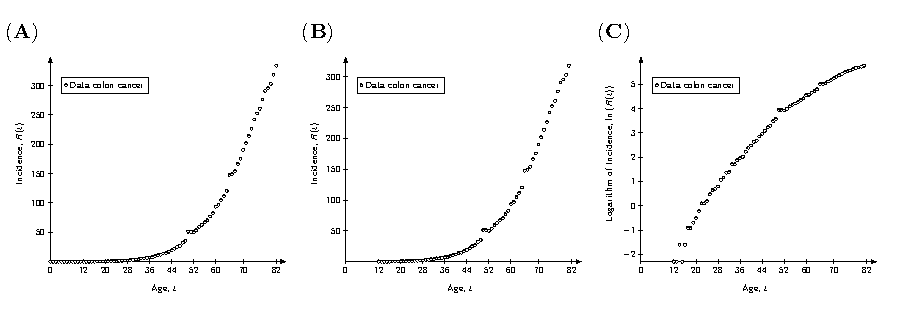
\includegraphics[width=\textwidth]{FigS4}
  \caption[Processing of the data]{\textit{Processing of the data}. The processing of the original data of the incidences of Myeloma in (\textbf{A}) is conducted in two steps. (\textbf{B}) Remove all zero incidences corresponding to all ages below 25 years. More precisely, this corresponds to the removal of the first 25 data points in the original time series. (\textbf{C}) Apply the logarithm to the incidences so that $\ln\left(R(t)\right)$ is reported as a function of the age $t$.}
  \label{fig:data_processing}
  \end{figure}

  The logarithmic version of the PLM given by

  $$R(t)=At^{\gamma}$$
  is given by
  $$\ln\left(R(t)\right)=\ln(A)+\gamma\ln(t).$$
  The logarithmic version of the IM-II given by
  $$R(t)=\dfrac{A}{\exp\left(e^{-\alpha(t-\tau)}\right)-1}$$
  is given by
  $$\ln\left(R(t)\right)=\ln(A)-\ln\left(\exp\left(e^{-\alpha(t-\tau)}\right)-1\right).$$
  Again, it is the logarithmic versions of the models that are fitted to the processed data (Fig \ref{fig:data_processing}C).


  The fit of each model is evaluated based on the \textit{adjusted $R^2$ value} denoted by $R^2_{\mathrm{adj}}$. If $n$ corresponds to the number of data points in the time series and $k$ corresponds to the number of parameters in each model then this value is defined as follows

    $$R^2_{\mathrm{adj}}=1-\left[\dfrac{\left(1-R^2\right)\left(n-1\right)}{n-k-1}\right]$$
    where\vspace{-0.3cm}
    $$R^2=1-\dfrac{\sum\limits_{i=1}^{n}\left(\ln\left(R_i\right)-\ln\left(\tilde{R}(t_i)\right)\right)^2}{\sum\limits_{i=1}^{n}\left(\ln\left(R_i\right)-\overline{R}\right)^2}=1-\dfrac{\textrm{Variation between model and data}}{\textrm{Internal variation in data}}.$$
In the above expression, $R_i$ corresponds to the data points, $\tilde{R}(t_i)$ corresponds to the output of the model and $\overline{R}$ is the mean value of the \textit{logarithmised data} (not the original data). The $R^2_{\mathrm{adj}}$ penalises the number of parameters, but as $\alpha$ is kept fixed in the fitting procedure the number of parameters is $k=2$ for both the PLM and the IM-II. Otherwise, the $R^2_{\mathrm{adj}}$ shares the following two properties with the $R^2$:


    \begin{enumerate}
    \item A perfect fit correponds to $R^2_{\mathrm{adj}}=1$,
      \item A really bad fit corresponds to $R^2_{\mathrm{adj}}<0$ which says that the model fits the data worse than a straight line.      
      \end{enumerate}
    
  

  